\everymath{\displaystyle}
\documentclass{beamer}
% \documentclass[handout]{beamer}

%\usepackage[pdftex]{color,graphicx}
\usepackage{amsmath,amssymb,amsfonts}

\mode<presentation>
{
  % \usetheme{Darmstadt}
  % \usetheme[hideothersubsections]{Hannover}
  % \usetheme[hideothersubsections]{Goettingen}
  \usetheme[hideothersubsections, right]{Berkeley}

  \usecolortheme{seahorse}
  % \usecolortheme{dolphin}
  \usecolortheme{rose}
  % \usecolortheme{orchid}

  \useinnertheme[shadow]{rounded}

  % \setbeamercovered{transparent}
  \setbeamercovered{invisible}
  % or whatever (possibly just delete it)
}

\mode<handout>{
  \setbeamercolor{background canvas}{bg=black!5}
  \usepackage{pgfpages}
  \pgfpagesuselayout{4 on 1}[a4paper,border shrink=5mm, landscape]
}

\usepackage[brazilian]{babel}
% or whatever

% \usepackage[latin1]{inputenc}
\usepackage[utf8]{inputenc}
% or whatever

\usepackage{times}
%\usepackage[T1]{fontenc}
% Or whatever. Note that the encoding and the font should match. If T1
% does not look nice, try deleting the line with the fontenc.


\title%[] % (optional, use only with long paper titles)
{Comparando médias de 2 grupos}

\subtitle
{Intervalos de Confiança da diferença entre as médias} % (optional)

\author%[] % (optional, use only with lots of authors)
{Felipe Figueiredo}% \and S.~Another\inst{2}}
% - Use the \inst{?} command only if the authors have different
%   affiliation.

\institute[] % (optional, but mostly needed)
{
}
  % \inst{1}%
  % Department of Computer Science\\
  % University of Somewhere
  % \and
  % \inst{2}%
  % Department of Theoretical Philosophy\\
  % University of Elsewhere}
% - Use the \inst command only if there are several affiliations.
% - Keep it simple, no one is interested in your street address.

\date%[] % (optional)
{}

% \subject{Talks}
% This is only inserted into the PDF information catalog. Can be left
% out. 



% If you have a file called "university-logo-filename.xxx", where xxx
% is a graphic format that can be processed by latex or pdflatex,
% resp., then you can add a logo as follows:

\pgfdeclareimage[height=1.6cm]{university-logo}{../logo}
\logo{\pgfuseimage{university-logo}}



% Delete this, if you do not want the table of contents to pop up at
% the beginning of each subsection:
\AtBeginSubsection[]
%\AtBeginSection[]
{
  \begin{frame}<beamer>{Sumário}
    \tableofcontents[currentsection,currentsubsection]
  \end{frame}
}


% If you wish to uncover everything in a step-wise fashion, uncomment
% the following command: 

% \beamerdefaultoverlayspecification{<+->}

\usepackage[normalem]{ulem}

\begin{document}

\begin{frame}
  \titlepage
\end{frame}

\begin{frame}{Sumário}
  \tableofcontents
  % You might wish to add the option [pausesections]
\end{frame}


%% Template
% \section{}

% \subsection{}

% \begin{frame}{}
%   \begin{itemize}
%   \item 
%   \end{itemize}
% \end{frame}

% \begin{frame}
%   \begin{columns}
%     \begin{column}{5cm}
%     \end{column}
%     \begin{column}{5cm}
%     \end{column}
%   \end{columns}
% \end{frame}

% \begin{frame}{}
%   \includegraphics[height=0.4\textheight]{file1}
%   \includegraphics[height=0.4\textheight]{file2}
%   \includegraphics[height=0.4\textheight]{file3}
%   \begin{figure}
%     \caption{}
%   \end{figure}
% \end{frame}

% \begin{frame}{}
%   \begin{definition}
%   \end{definition}
%   \begin{example}
%   \end{example}
%   \begin{block}{Exercício}
%   \end{block}
% \end{frame}

% \section{Discussão da aula passada}

% \subsection{Discussão da aula passada}

\begin{frame}{\scriptsize Discussão da aula passada}
  \begin{block}{}
    Discussão da leitura obrigatória da aula passada
  \end{block}
\end{frame}

\section[t de Student]{A distribuição t de Student}

\subsection{A distribuição t de Student}

\begin{frame}{\scriptsize Recapitulando}
  \begin{block}{\em Não vá se perder por aí...}
    \begin{itemize}
      \footnotesize
    \item A distribuição Normal tem {\bf dois} parâmetros
    \item Seu formato é absolutamente definido por
      \begin{itemize}
        \scriptsize
      \item $\bar{x}$ = Média {\tiny (tendência central)}
      \item $s^2$/$s$ = Variância/DP {\tiny (tendência de dispersão)}
      \end{itemize}
    \end{itemize}
    \begin{center}
      $\Rightarrow$ Forma \alert{independe} do $n$
    \end{center}
  \end{block}
  \begin{block}{Nomenclatura}<2->
    \small
    A {\em Normal Padrão} também é chamada de {\bf distribuição Z}.
  \end{block}
\end{frame}

\begin{frame}{\scriptsize Recapitulando}
  \begin{itemize}
    \footnotesize
  \item Vimos que o IC {\tiny(da média)} é composto por 3 componentes
    \begin{itemize}
      \scriptsize
    \item a média $\bar{x}$ {\tiny(centro)}
    \item o erro padrão da média -- SEM {\tiny(incerteza)}
    \item {\em um tal} de t$^{*}$, que depende de $n$
    \end{itemize}
  \item Quando $n$ era grande, utilizamos $t^{*} \approx 2$
    \bigskip
  \item Mas de onde vem esse $t^{*}$? Qual seria o valor \alert{correto}?
  \end{itemize}
\end{frame}

\begin{frame}{\scriptsize A distribuição t de Student}
  \begin{center}
    
\includegraphics[height=\textheight]{Cap5/Guinness}
  \end{center}
\end{frame}

\begin{frame}{\scriptsize A distribuição t de Student}
  \begin{center}
    
\includegraphics[height=\textheight]{Cap5/Student-Guinness}
  \end{center}
\end{frame}

\begin{frame}{\scriptsize A distribuição t de Student}
  \begin{itemize}
    \footnotesize
  \item Student (pseudônimo de W. S. Gossett [1876-1937]\footnote{trabalhando
    para a cervejaria Guiness})
  \item Distribuição {\bf t} ({\footnotesize baseada na distribuição Normal})
  \item Melhor se aproxima dos dados de {\em amostras pequenas}
%  \item É semelhante à Normal padrão, mas tem variância maior
  \item 3$^o$ parâmetro \alert{graus de liberdade}\footnote{df em inglês} {\footnotesize vinculado ao tamanho da amostra $n$}.
    % \begin{displaymath}
    %   gl = n-1
    % \end{displaymath}
  \end{itemize}
\end{frame}

\begin{frame}{\scriptsize Propriedades da distribuição t}
  \begin{itemize}
    \footnotesize
  \item A distribuição tem forma de sino {\footnotesize(simétrica, como a Normal)}
  \item Reflete a maior variabilidade \alert{inerente} às amostras pequenas\footnote{graus de liberdade (df) $\approx$ $n$}
  \item Formato {\em depende} do tamanho da amostra ($n$) %\footnote{A distr. Normal depende apenas de $\mu$ e $\sigma$}
  \end{itemize}
  \begin{block}{Isto é}
    \footnotesize
    Quanto mais graus de liberdade, mais a distribuição $t$ se parece com a distribuição Normal ($Z$)
  \end{block}
  \begin{block}{Pense...}<2->
    \footnotesize
    O que deve acontecer com \alert{menos} graus de liberdade?
  \end{block}
\end{frame}

\begin{frame}{\scriptsize A distribuição t de Student}
  \begin{figure}
    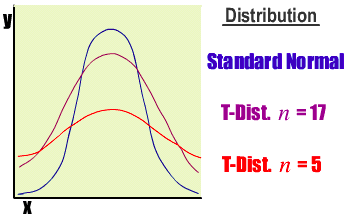
\includegraphics[height=0.7\textheight]{Cap7/t_graph}
    \caption{\footnotesize Duas distribuições t de Student, e a Normal padrão}
  \end{figure}
\end{frame}

% \begin{frame}{\scriptsize A tabela t}
%   \begin{center}
%     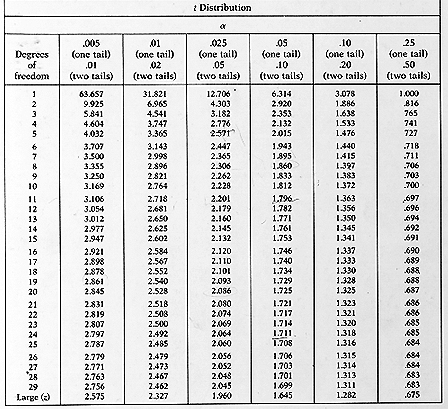
\includegraphics[height=0.9\textheight]{Cap7/t_table}
%   \end{center}
% \end{frame}


\begin{frame}{\scriptsize IC da média (aula passada)}
  \begin{exampleblock}{ICs dos exemplos}
    \footnotesize
    \begin{itemize}
      \footnotesize
    \item IC do ex. 5.1 (PS de 100 alunos): [120.6, 126.2] mmHg
    \item IC do ex. 5.2 (PS de   5 alunos): [79.2, 118.8] mmHg
    \end{itemize}
  \end{exampleblock}
  \begin{block}{Pense...}
    Observe os tamanhos dos ICs.
  \end{block}
  \begin{block}{Lembrete}<2->
    Para o 5.1, usamos $t^{*} \approx$ 2.

    \bigskip
    Vimos que esta aproximação \alert{não era apropriada} no 5.2
  \end{block}

\end{frame}

\begin{frame}{\scriptsize Alguns valores de $t^{*}$, para diferentes graus de liberdade}
  \begin{itemize}
    \footnotesize
  \item $n = 5\ (df = 4) \Rightarrow t^{*} = 2.776$
  \item $n = 10\ (df = 9) \Rightarrow t^{*} = 2.262$
  \item $n = 15\ (df = 14) \Rightarrow t^{*} = 2.145$
  \item $n = 20\ (df = 19) \Rightarrow t^{*} = 2.093$
  \item $n = 30\ (df = 29) \Rightarrow t^{*} = 2.045$
  \end{itemize}
  \begin{block}{Pense...}
    \footnotesize
    Qual é a relação entre $n$ e o tamanho do IC?

    % \begin{displaymath}
    %   IC: \bar{x} \pm t^{*} \times SEM
    % \end{displaymath}
    \begin{displaymath}
      IC = \left[ \bar{x} - t^{*} SEM,\ \ \bar{x} + t^{*} SEM \right]
    \end{displaymath}
  \end{block}
\end{frame}

\begin{frame}{\scriptsize Alguns valores de $t^{*}$, para diferentes graus de liberdade}
  \begin{itemize}
    \footnotesize
  \item $n = 5\ (df = 4) \Rightarrow t^{*} = 2.776$
  \item $n = 10\ (df = 9) \Rightarrow t^{*} = 2.262$
  \item $n = 15\ (df = 14) \Rightarrow t^{*} = 2.145$
  \item $n = 20\ (df = 19) \Rightarrow t^{*} = 2.093$
  \item $n = 30\ (df = 29) \Rightarrow t^{*} = 2.045$
  \end{itemize}
  \begin{block}{Observe que...}
    \footnotesize
    \begin{itemize}
      \scriptsize
    \item $df = n - 1$
    \item Para $n$ grande, $t^{*} \rightarrow 1.960$
    \end{itemize}
    \bigskip
    \scriptsize
    {\em Por isso} usamos o valor aproximado $2$ no primeiro exemplo.
  \end{block}
\end{frame}

\begin{frame}{\scriptsize Na prática...}
  \begin{block}{Distribuição Normal - Z}
    \footnotesize
    {\em Gostaríamos} de poder usar sempre Z como \alert{modelo} para o formato dos nossos dados experimentais.
  \end{block}
  \begin{block}{Distribuição t de Student}
    \begin{itemize}
      \footnotesize
    \item t é uma aproximação da Normal (Z)
      \medskip
    \item idealizada para $n$ pequeno
      \medskip
    \item Com $n$ grande (df $\ge 30$) ela {\em se confunde} com Z.
    \end{itemize}
  \end{block}
\end{frame}

\begin{frame}[label=exercicio5.4]{\scriptsize Exercício 4 (cap 5)}
  \begin{exampleblock}{Exercício 4 do cap 5}
    \footnotesize
    Os níveis séricos de um hormônio (fator Y) foram medidos em 100 mulheres não grávidas, e em 100 mulheres com até 3 meses de gravidez.
    Os ICs dos valores dos soros em ambos os grupos são:
    \begin{itemize}
      \footnotesize
    \item Grávidas: [105.4, 114.6]
    \item Não grávidas: [90.0, 96.0]
    \end{itemize}

    \bigskip
    {\bf O fator Y médio é diferente em mulheres grávidas e não grávidas?}
  \end{exampleblock}
  \begin{block}{Requisito}<2->
    \footnotesize
    Pelas premissas do IC da média, você tem informações suficientes para calcular/interpretar cada um destes ICs?
  \end{block}
\end{frame}

\begin{frame}{\scriptsize Pense}
    \footnotesize
  \begin{exampleblock}{Exercício 5.4}
    \footnotesize
    \begin{itemize}
      \footnotesize
    \item Não grávidas: [90.0, 96.0]
    \item Grávidas: [105.4, 114.6]
    \end{itemize}
  \end{exampleblock}
  \bigskip
  Observações:
  \begin{itemize}
    \footnotesize
  \item {\small O SEM informa {\em quão bem você estimou a média} de cada grupo}
  \item {\small Os ICs não tem sobreposição $\Rightarrow$ 2 populações diferentes}
  \end{itemize}
  \bigskip
  \begin{block}{Pense...}
    \begin{center}
      Como comparar estes dois grupos?
    \end{center}
  \end{block}
\end{frame}

\section[IC diferença 2 médias]{Intervalo de Confiança da diferença entre duas médias}

\subsection{Interpretação}

\begin{frame}{\scriptsize Comparações entre 2 médias}
  \begin{itemize}
    \footnotesize
  \item Frequentemente precisamos dividir os dados em dois grupos e
    comparar as médias.

    \bigskip
  \item Isto pode ser usado para se estudar o efeito de um tratamento
    em relação a um grupo controle

    \bigskip
  \item ou mesmo para se comparar dois tratamentos diferentes.
  \end{itemize}
\end{frame}

\againframe{exercicio5.4}

\begin{frame}{\scriptsize Quais são as variáveis?}
  \begin{itemize}
    \footnotesize
  \item $x_C$ Hormônio não grávidas
  \item $x_T$ Hormônio grávidas (até 3 meses)
  \item Duas variáveis explícitas
  \end{itemize}
  \begin{block}{Primeira alternativa}
    \small
    \begin{enumerate}
      \footnotesize
    \item``Explicar'' a ``relação'' entre o hormônio $x_T$ e o hormônio $x_C$% como ``referência''
    \item Comparar $x_T$ (grupo de teste) com $x_C$ (referência)%\footnote{valor médio!}
    \end{enumerate}
  \end{block}
  \begin{block}{Esta relação pode ser expressa como}
    \begin{displaymath}
      x_T \sim x _C
    \end{displaymath}
  \end{block}
\end{frame}

\begin{frame}{\scriptsize Uma breve interrupção para mini-pânico}
  \vfill
  \vfill
  \vfill
  \vfill
  \vfill
  \hfill \small Suspense dramático...
\end{frame}

\begin{frame}{\scriptsize Uma breve interrupção para mini-pânico}
  \begin{block}{Se você prestou atenção até aqui...}
    Temos \alert{duas} variáveis.

    Portanto temos duas médias (trivial).

    \bigskip
    Mas também temos \alert{dois SEM}!
  \end{block}
  \begin{block}{Esta relação pode ser expressa como}
    \begin{displaymath}
      \text{horm. grávidas} \sim \text{horm. não grávidas}
    \end{displaymath}
  \end{block}
  \begin{block}{Mais precisamente}
    \begin{displaymath}
      \text{horm. grávid.} = \text{horm. não grávid.} + \alert{\text{Erro}_C + \text{Erro}_T}
    \end{displaymath}
  \end{block}
\end{frame}

\begin{frame}{\scriptsize Uma breve interrupção para mini-pânico}
  \begin{center}
    
\includegraphics[height=.7\textheight]{Cap7/ogrito}
  \end{center}
  \begin{block}{}
    \begin{center}
      Duas médias, e dois erros?
    \end{center}
  \end{block}
\end{frame}

\begin{frame}{\scriptsize Duas opções}
  \begin{exampleblock}{Exercício 5.4}
    \footnotesize
    \begin{itemize}
      \footnotesize
    \item Não grávidas: [90.0, 96.0]
    \item Grávidas: [105.4, 114.6]
    \end{itemize}
  \end{exampleblock}
  \begin{block}{Difícil}
    Calcular os dois ICs ($x_C$ e $x_T$), e compará-los diretamente
  \end{block}
  \begin{block}{Moleza}
    \only<1>{Calcular o IC da diferença ($x_d$) usando o método da aula passada}
    \only<2>{\bf Calcular o IC da diferença ($x_d$) usando o método da aula passada}
  \end{block}
\end{frame}

\begin{frame}{\scriptsize }
  \begin{block}{}
    \large
    Neste caso podemos usar um truque para \alert{trocar} um problema de 2 variáveis por outro de 1 variável.
  \end{block}
  \bigskip
  \bigskip
  \begin{center}
    
\includegraphics[width=.6\textwidth]{Cap7/magic}
  \end{center}
\end{frame}

\begin{frame}{\scriptsize 2 grupos {\em for dummies} \textregistered}
  \begin{block}{Diferença entre 2 médias}
    \begin{itemize}
      \scriptsize
    \item Comparar duas médias $\bar{x_C}$ e $\bar{x_T}$, consideramos a diferença média $\bar{x_d} = \bar{x_T} - \bar{x_C}$
    \item<2-> Se $\bar{x_T}$ for maior que $\bar{x_C}$  $\Rightarrow$ diferença média é positiva
    \item<2-> Se $\bar{x_T}$ for menor que $\bar{x_C}$  $\Rightarrow$ a diferença média é negativa
    \end{itemize}
  \end{block}
  \begin{block}{Intuição}
    Raciocínio: se as médias forem aproximadamente iguais, {\bf a
    diferença média ($\bar{x_d}$) será próxima de zero}
  \end{block}
  \bigskip
  \begin{center}
    {\em Pense em \alert{saldo}}
    \footnotesize
  \end{center}
\end{frame}

\begin{frame}{\scriptsize Quais são as variáveis?}
  \begin{itemize}
    \footnotesize
  \item $x_C$ Hormônio não grávidas
  \item $x_T$ Hormônio grávidas (até 3 meses)
  \item $d = x_T - x _C$ (uma variável)
  \end{itemize}
  \begin{block}{Segunda alternativa (método da aula passada)}
    \footnotesize
    ``Explicar'' a ``relação'' entre a diferença $d$ e a referência ({\bf zero})
  \end{block}
  \begin{block}{Esta relação pode ser expressa como}
    \footnotesize
    \begin{displaymath}
      d \sim 0
    \end{displaymath}
  \end{block}
\end{frame}

\begin{frame}{\scriptsize Quais são as variáveis?}
  \begin{block}{Estratégia proposta}
    \footnotesize
    Temos duas variáveis.

    \bigskip
    Calculamos a \alert{diferença} entre as médias e aplicamos o método da aula passada -- IC de {\bf uma} média.

    \begin{center}
      moleza!
    \end{center}
  \end{block}
  \begin{center}
    \footnotesize
    O que falta?
  \end{center}
  \begin{block}{O que falta?}<2->
    ... precisamos do {\em SEM da diferença}.
  \end{block}
  \begin{block}{Ou seja...}<3->
    \begin{displaymath}
      d = 0 + \alert{Erro_d}
    \end{displaymath}
  \end{block}

\end{frame}

\begin{frame}{\scriptsize Uma breve interrupção para mini-pânico}
  \begin{center}
    
\includegraphics[height=.7\textheight]{Cap7/ogrito}
  \end{center}
  \begin{block}{}
    \begin{center}
      SEM da diferença?
    \end{center}
  \end{block}
\end{frame}

\begin{frame}{\scriptsize Erro padrão da diferença}
  \begin{itemize}
    \footnotesize
  \item Lembre-se que para cada grupo: $SEM = \frac{s}{\sqrt{n}}$
  \item Para a diferença entre 2 grupos, ``somamos'' os SEM
  \item Mas esta ``soma'' não é direta!
  \item É preciso levar em conta o uso do quadrado/raiz quadrada do DP (aula de variabilidade\footnote{não podemos somar DPs, mas podemos somar variâncias})
  \end{itemize}
  \begin{block}{}
      \begin{displaymath}
    SE = \sqrt{SEM_1^2 + SEM_2^2}
  \end{displaymath}
  \end{block}
\end{frame}

\begin{frame}{\scriptsize De volta à programação normal}
  \begin{center}
    
\includegraphics[height=.7\textheight]{Cap7/naoentreempanico}
  \end{center}
    \begin{block}{Estratégia proposta}
      \begin{center}
        {\em SEM da diferença}.
      \end{center}
  \end{block}
\end{frame}

\begin{frame}{\scriptsize Premissas}
  \begin{itemize}
    \footnotesize
  \item As amostras foram selecionadas aleatoriamente das respectivas populações
  \item As populações são Normais (Gaussianas)
  \item As duas populações possuem DP idênticos
  \item Todos os indivíduos de cada grupo vêm da mesma população
  \item Cada indivíduo é independente de todos os outros
  \end{itemize}
\end{frame}

\againframe{exercicio5.4}

\begin{frame}{\scriptsize Bastidores do exercício 5.4/7.1}
  \begin{exampleblock}{Diferenças: Exercício 5.4 (e 7.1)}
    \footnotesize
    \begin{exampleblock}{}
    \footnotesize
      \begin{itemize}
        \footnotesize
      \item {\scriptsize Média grávidas: $\bar{x_C} = 110$ unidades/ml}
      \item {\scriptsize Média não grávidas: $\bar{x_T} = 93$ unidades/ml}
      \item Diferença entre as médias: $\bar{x_d} = \alert{17}$ unidades/ml
      \end{itemize}
    \end{exampleblock}
    \begin{exampleblock}{}
    \footnotesize
      \begin{itemize}
        \footnotesize
      \item SEM da diferença: \alert{2.75} unidades/ml
      \end{itemize}
    \end{exampleblock}
    \begin{exampleblock}{}
    \footnotesize
      \begin{itemize}
        \footnotesize
      \item {\scriptsize $n_C$ = 100, $n_T$ = 100}
      \item df = (100 -1) + (100 - 1) = \alert{198}
      \end{itemize}
    \end{exampleblock}
    \begin{exampleblock}{}
    \footnotesize
      \begin{itemize}
        \footnotesize
      \item $t^{*} = \alert{1.97}$ {\tiny(valor crítico tabelado)}
      \end{itemize}
    \end{exampleblock}
  \end{exampleblock}
\end{frame}

\begin{frame}{\scriptsize Solução do exercício 5.4/7.1}
  \begin{exampleblock}{Bastidores: Exercício 5.4 (e 7.1)}
    \tiny
    \begin{itemize}
    \item Média grávidas: $\bar{x_C} = 110$ unidades/ml
    \item Média não grávidas: $\bar{x_T} = 93$ unidades/ml
    \item Diferença entre as médias: $\bar{x_d} = \alert{17}$ unidades/ml
    \item SEM da diferença: \alert{2.75} unidades/ml
    \item $n_C$ = 100, $n_T$ = 100
    \item df = (100 -1) + (100 - 1) = \alert{198}
    \item $t^{*} = \alert{1.97}$ {\tiny(valor crítico tabelado)}
    \end{itemize}
  \end{exampleblock}
  \begin{exampleblock}{Resultado: IC da diferença}
    \footnotesize
    \centering
    {\bf [11.6, 22.4] unidades/ml}
  \end{exampleblock}
  \begin{center}
    \scriptsize
    {\em E o que isso significa?}
  \end{center}
\end{frame}

\begin{frame}{\scriptsize Solução}
  %   \begin{exampleblock}{IC}
  %   \centering
  %   [11.6, 22.4] unidades/ml
  % \end{exampleblock}
  \begin{exampleblock}{Interpretação}
    Estamos 95\% {\em confiantes} que a diferença \alert{real} entre os grupos está entre 11,6 e 22,4.
    \scriptsize
  \end{exampleblock}

  \bigskip
  \begin{exampleblock}{Conclusão {(\em ``nossos dados indicam que...'')}}
    \small
    o (...) fator Y de uma (...) grávida é (...) 17 unidades/ml maior que uma (...) não grávida (variando entre 11,6 e 22,4 unidades/ml).
  \end{exampleblock}
  \begin{block}{Pense...}<2->
    \scriptsize
    Preencha as lacunas acima.
  \end{block}
\end{frame}

\subsection{Participantes: pareados ou não pareados?}

\begin{frame}{\scriptsize Grupos não pareados x pareados}
  \begin{block}{Grupos não pareados}
    \begin{itemize}
      \footnotesize
    \item Até agora assumimos que os grupos e participantes são {\bf independentes}
    \item A única coisa que podemos fazer: {\bf comparação global}
    \item ... a média do grupo A $\times$ a média do grupo B
    \end{itemize}
  \end{block}
  \begin{block}{Grupos pareados}
    \begin{itemize}
      \footnotesize
    \item Existe um caso importante em que pode-se considerar que eles são dependentes: quando são pareados
    \item Isto é: cada participante de um grupo tem um correspondente no outro
    \item ... diferença entre cada par $\Rightarrow$ média das diferenças
    \end{itemize}
  \end{block}
\end{frame}

\begin{frame}{\scriptsize Grupos pareados}
  \scriptsize
Quando faz sentido parear indivíduos de dois grupos?
  \bigskip
  \begin{itemize}
    \scriptsize
  \item Mensurar o \alert{mesmo} individuo antes e depois do procedimento ({\em baseline} x intervenção)
    \medskip
  \item Recrutamento aos pares, quando o par tem a(o) mesma(o)
    \begin{itemize}
      \tiny
    \item idade/faixas etária
    \item região demográfica
    \item diagnóstico
    \end{itemize}
    \medskip
  \item irmãos, pai/filho
    \medskip
  \item lateralidade (tratamento = lado E, controle = lado D)
  \end{itemize}
\end{frame}

\begin{frame}{\scriptsize Qual das estimativas é mais precisa?}
  \begin{exampleblock}{Exemplo 7.2}
    \scriptsize
    Ye e Grantham (1993) estudaram o mecanismo de absorção de fluido em cistos renais removidos de pacientes com doença renal policística.
    Incubaram os cistos em meio de cultura celular e mediram a diferença de peso em cada cisto (antes e depois da incubação).

    \scriptsize
    \begin{exampleblock}{Não pareado}
      \footnotesize
      \begin{enumerate}
        \footnotesize
      \item<2,4> peso médio (todos, antes) = 6.51g (SEM 2.26g)
      \item<2,4> peso médio (todos, depois) = 7.02g (SEM 2.40g)
      \item<2,4> IC 95\% [-6.48, 7.50]
      \end{enumerate}
    \end{exampleblock}
    \begin{exampleblock}{Pareado}
      \footnotesize
      \begin{enumerate}
        \footnotesize
      \item<3,4> ganho em {\bf cada} cisto $\Rightarrow$ depois - antes
      \item<3,4> ganho médio dos cistos = 0.50g (SEM 0.23g).
      \item<3,4> IC 95\% [-0.03, 1.04]
      \end{enumerate}
    \end{exampleblock}
  \end{exampleblock}
\end{frame}

\begin{frame}{\scriptsize IPC}
  \begin{block}{}
    A escolha entre grupos pareados e grupos não pareados é estratégica (planejamento do estudo), e não uma questão de ``preferência''.
  \end{block}
\end{frame}
\section{Aprofundamento}

\subsection{Aprofundamento}

\begin{frame}{\scriptsize Aprofundamento}
  \begin{block}{Leitura obrigatória}
    \begin{itemize}
      \footnotesize
    \item Capítulo 5. Seção: A distribuição {\em t}
    \item Capítulo 7: Pular as seções
      \begin{itemize}
        \scriptsize
      \item Cálculo do IC de grupos independentes
      \item Cálculo do IC de grupos pareados
      \end{itemize}
    \end{itemize}
  \end{block}
  \begin{block}{Leitura recomendada}
    \begin{itemize}
    \scriptsize
    \item {\bf ICH} - {\bf E10} Choice of Control Group in Clinical
      Trials
    \begin{itemize}
      \tiny
    \item Seção {\bf 2.1} ({\em Placebo Control})
    \item Cap. {\bf 3} ({\em CHOOSING THE CONCURRENT CONTROL GROUP})
    \end{itemize}
  \end{itemize}
    \hfill \scriptsize \href{http://www.ich.org/products/guidelines/efficacy/efficacy-single/article/choice-of-control-group-and-related-issues-in-clinical-trials.html}{http://www.ich.org} {\tiny (este link é clicável)}
  \end{block}
\end{frame}

\end{document}
